\section{问题五：最大恒定速度的求解}
\subsection{模型建立}
问题五要求在问题四给定调头路径上，确定龙头前把手可采用的最大恒定速度，并保证任一把手速度均不超过2 m/s。与前四问不同，本问不再改变几何路径，而是在既定路径上讨论速度约束；因此核心是把全队速度响应转化为龙头速度的比例放大问题。

设单位头速下第$i$个把手在时刻$t$的速度为$v_i^{(1)}(t)$。当龙头恒定速度由1 m/s改为$v_H$时，路径形状和各把手间距约束不变，时间尺度按同一比例缩放，故各把手速度满足
\[
v_i(t;v_H)=v_H\,v_i^{(1)}(t),
\]
从而速度约束可写为
\[
\max_{i,t} v_i(t;v_H)\le 2.
\]
于是最大头速满足
\[
v_{\max}=\frac{2}{\max_{i,t} v_i^{(1)}(t)}.
\]
该式把“所有把手速度均受限”的多变量约束，化为单位头速下最大速度放大倍数的计算。后续只需先求出速度矩阵$\{v_i^{(1)}(t)\}$，再由其中的最大值反推龙头速度上界。

\subsection{速度递推与约束转化}
设第$i-1$个把手与第$i$个把手之间的连杆方向单位向量为$\bm e_i$，两把手所在路径处的切向单位向量分别为$\bm \tau_{i-1}$和$\bm \tau_i$。由相邻把手距离约束对时间求导，可得沿连杆方向的速度投影相等：
\[
v_{i-1}(\bm \tau_{i-1}\cdot \bm e_i)
=v_i(\bm \tau_i\cdot \bm e_i).
\]
因此，在单位龙头速度$v_0=1$ m/s下，可逐节递推
\[
v_i^{(1)}(t)
=v_{i-1}^{(1)}(t)
\left|
\frac{\bm \tau_{i-1}\cdot \bm e_i}
{\bm \tau_i\cdot \bm e_i}
\right|.
\]
对所有$i=0,1,\ldots,223$和$t=-100,-99,\ldots,100$ s计算$v_i^{(1)}(t)$，即可得到速度放大倍数
\[
\lambda_{\max}=\max_{i,t} v_i^{(1)}(t).
\]
为定位约束最紧的位置和时刻，进一步定义
\[
M(t)=\max_i v_i^{(1)}(t),\qquad
G_i=\max_t v_i^{(1)}(t).
\]
其中$M(t)$反映每一时刻全队速度上界的变化，$G_i$反映各把手在整个调头过程中的最大速度放大情况。前者用于定位限制时刻，后者用于解释限制把手来源。

基于$M(t)$可绘制全队最大把手速度随时间变化图，用于说明速度约束如何在调头过程中形成。

\begin{figure}[H]
\centering
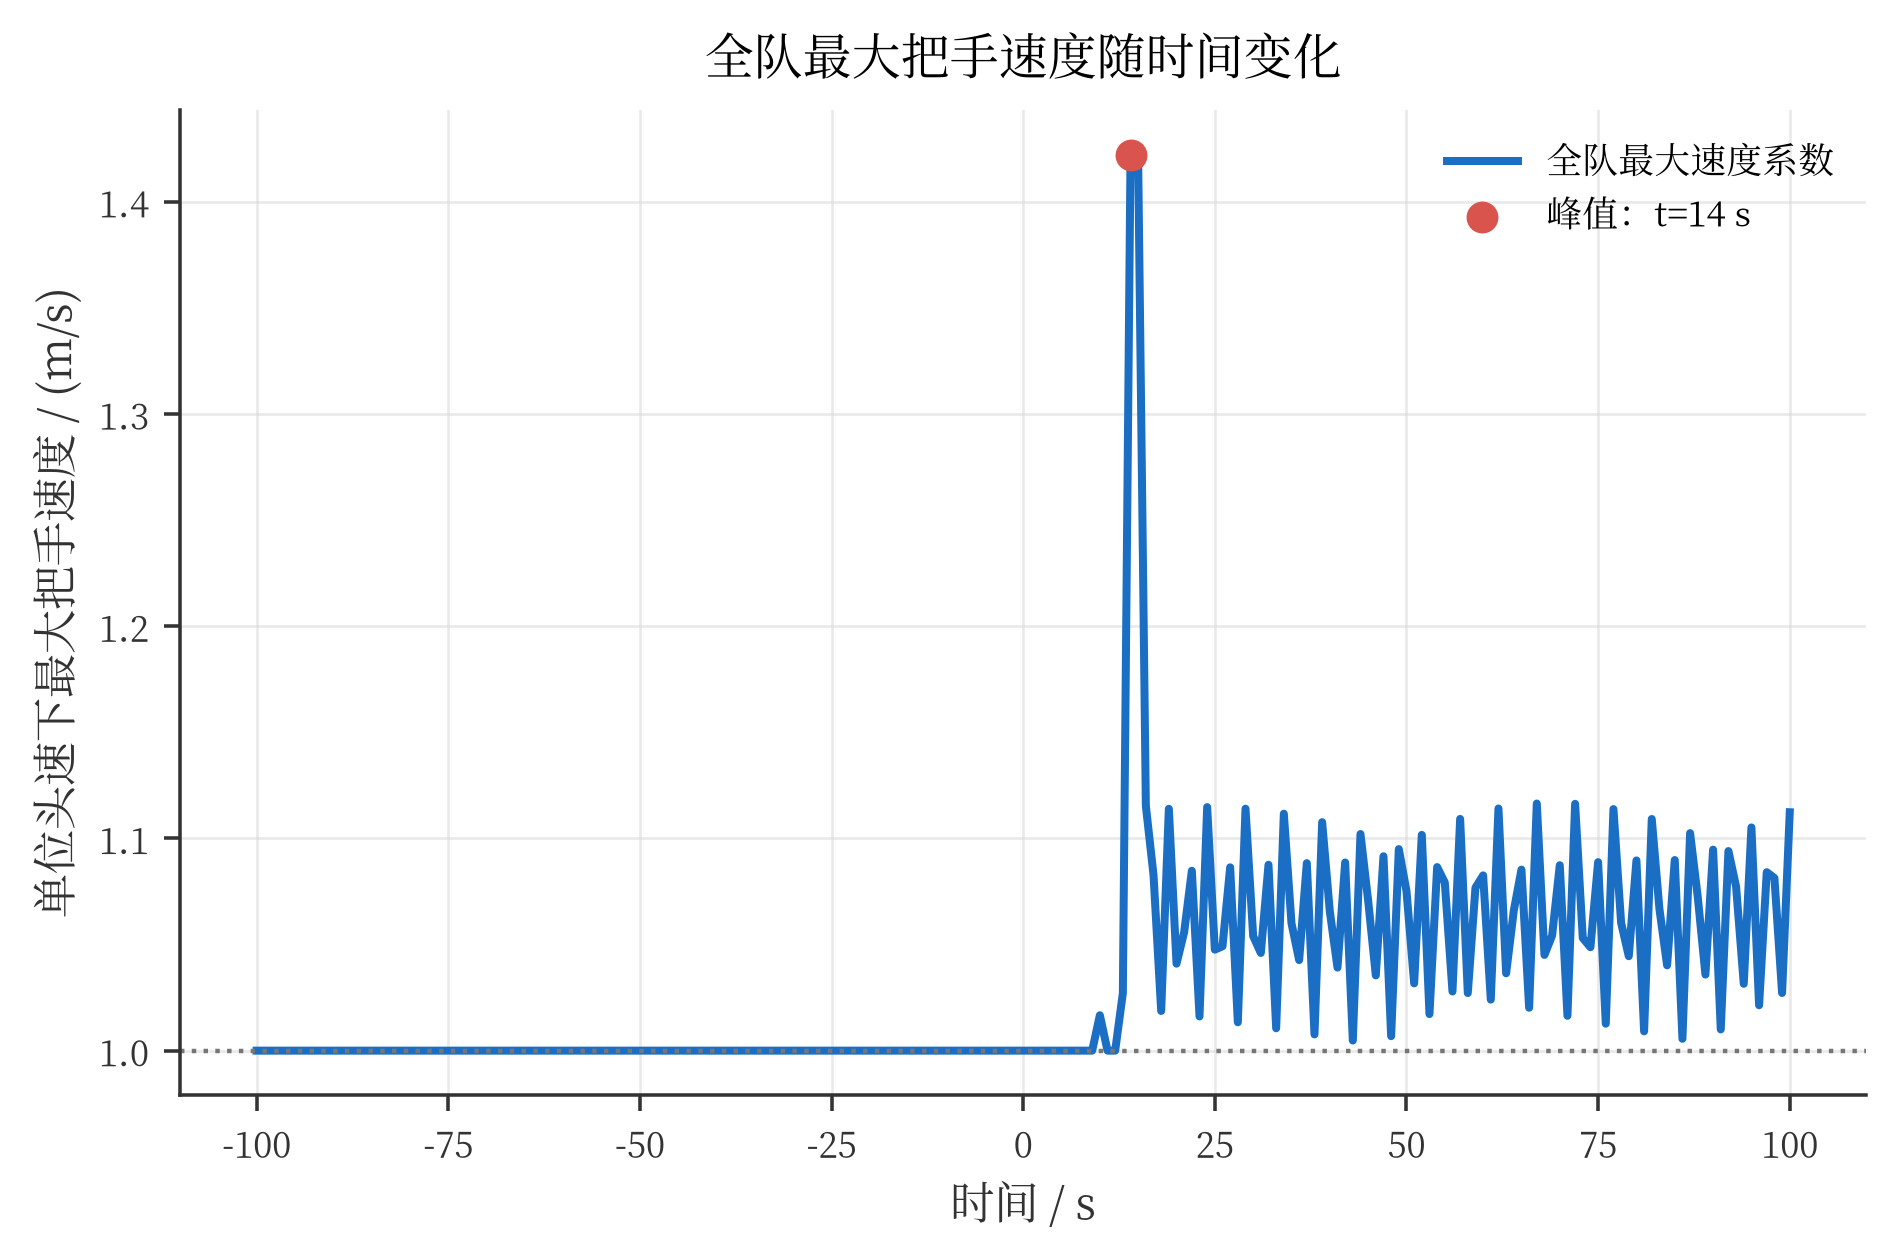
\includegraphics[width=0.88\textwidth]{figures/python/q5_time_max_speed.png}
\caption{单位头速下全队最大把手速度随时间变化}
\label{fig:q5-max-speed-time}
\end{figure}

进一步把速度放大倍数按“把手编号--时刻”展开，可得到单位头速下的速度放大倍数热力图，用于同时观察限制时刻与限制把手的位置。

\begin{figure}[H]
\centering
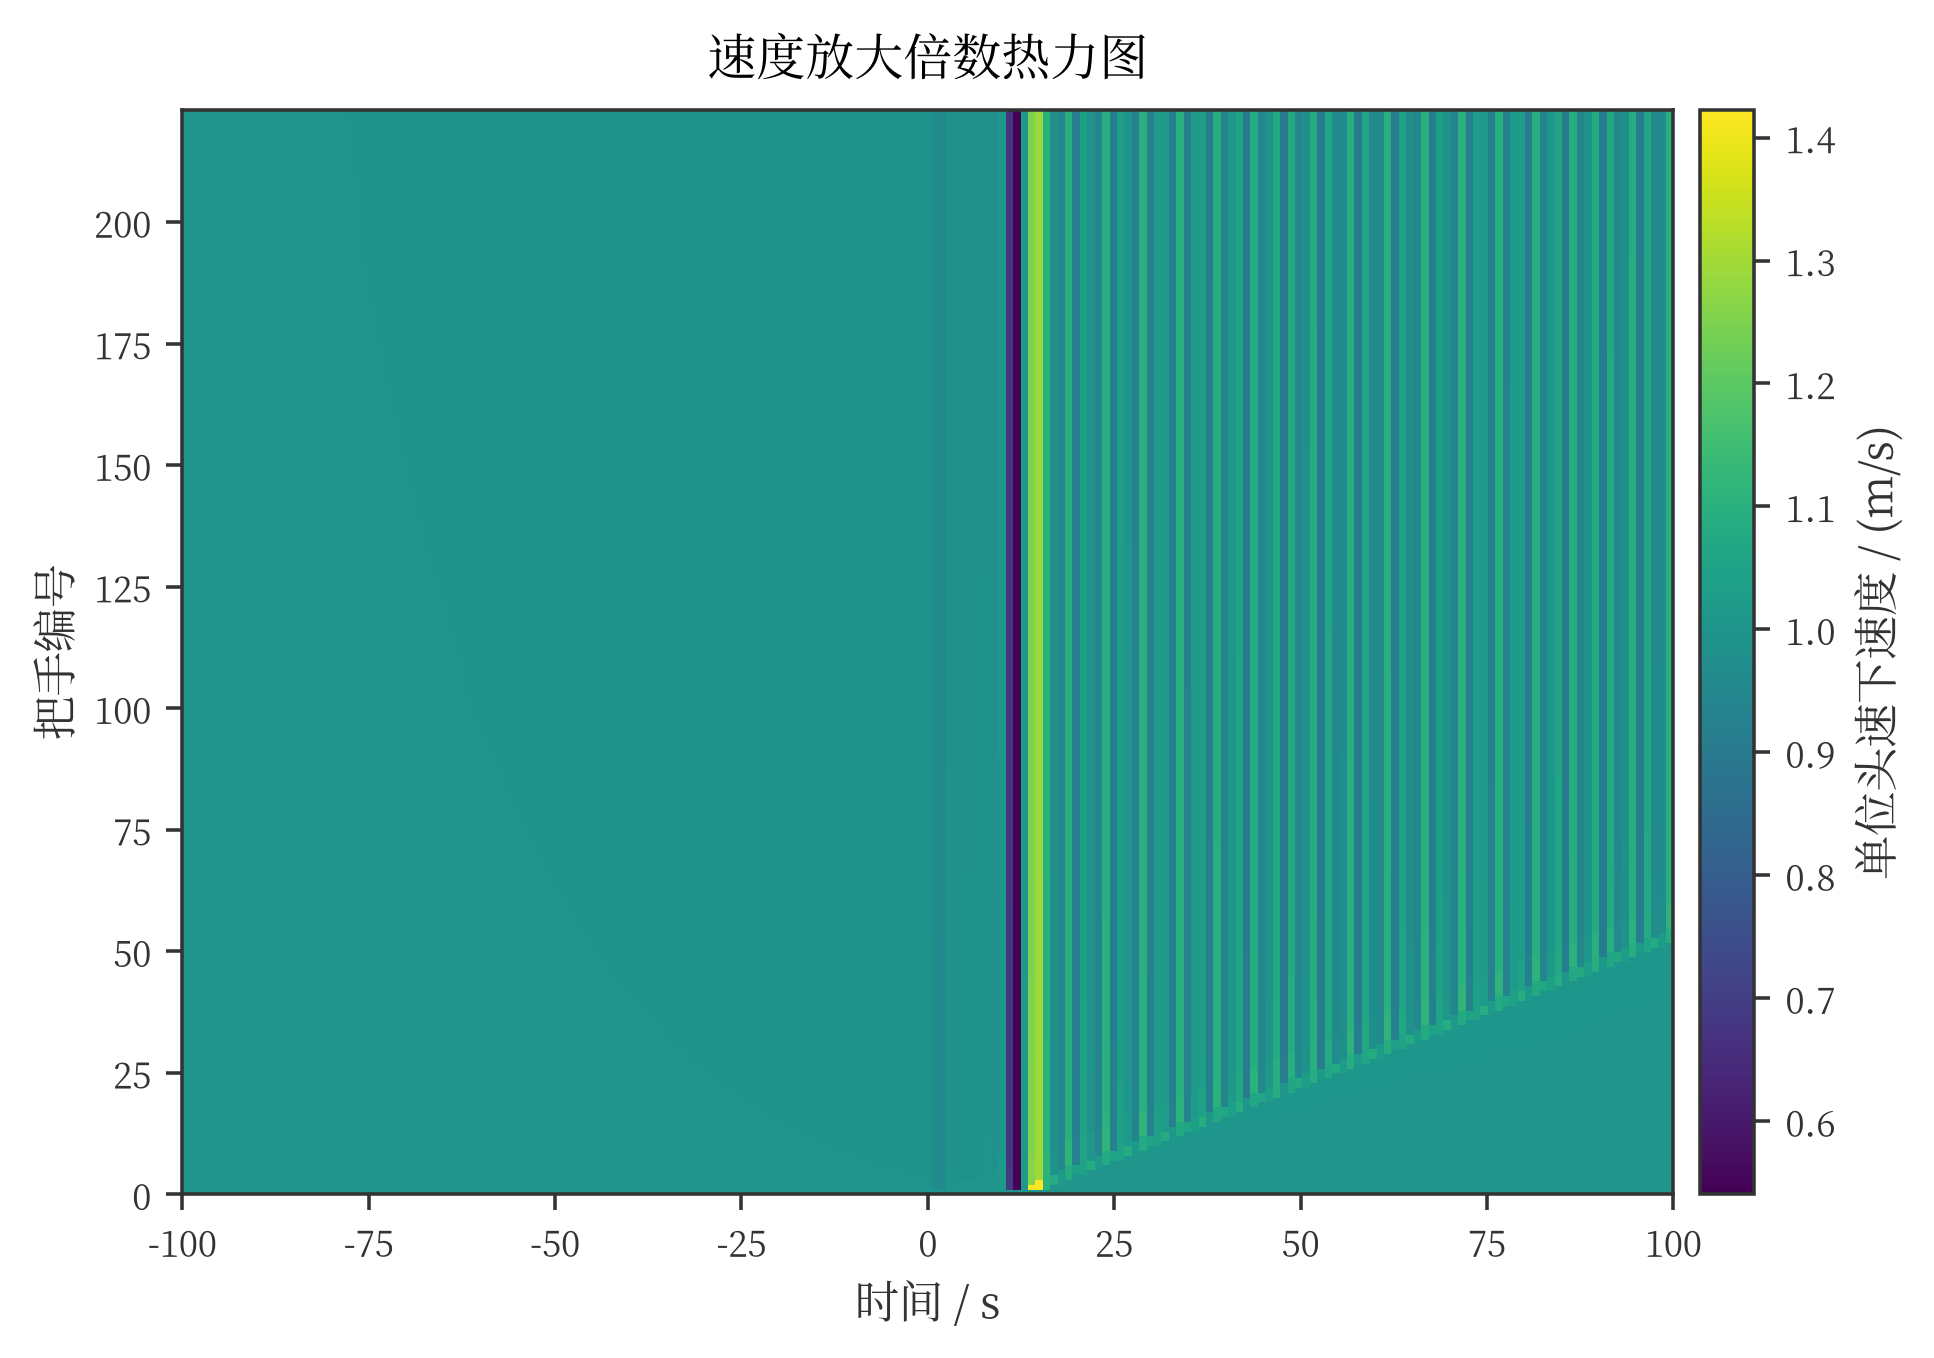
\includegraphics[width=0.9\textwidth]{figures/python/q5_speed_factor_heatmap.png}
\caption{单位头速下速度放大倍数热力图}
\label{fig:q5-speed-factor-heatmap}
\end{figure}

\subsection{求解过程}
求解时，首先读取问题四已经确定的固定交点复合路径；随后在$-100$到$100$ s的整数时刻上，按相邻把手距离约束递推全部把手位置；再根据切向投影关系计算单位头速下的速度矩阵。最后从该矩阵中提取$\lambda_{\max}$、限制时刻和限制把手，并代入$v_{\max}=2/\lambda_{\max}$得到龙头速度上界。

\begin{algorithm}[H]
\caption{问题五最大恒定头速反推流程}
\label{alg:q5-speed}
\textbf{Input:} 问题四固定调头路径，最大允许把手速度$2$ m/s。\\
\textbf{Output:} 龙头最大恒定速度$v_{\max}$。
\begin{enumerate}[label=\arabic*:, leftmargin=2.6em, itemsep=0.2em]
\item 由固定交点和两段相切圆弧构造复合路径。
\item 对每个整数时刻$t\in[-100,100]$，递推求解全部把手位置。
\item 在单位头速下递推计算各把手速度。
\item 取速度矩阵中的最大值作为$\lambda_{\max}$。
\item 根据$v_{\max}=2/\lambda_{\max}$反推龙头速度上界。
\item \textbf{return} $v_{\max}$。
\end{enumerate}
\end{algorithm}

\subsection{结果分析}
最终得到的最大恒定头速为
\[
v_{\max}=1.406\ \text{m/s},
\]
对应最大放大倍数为$1.422$。在该速度下，全队最大把手速度为
\[
2.000\ \text{m/s},
\]
满足题目要求。

单位头速速度矩阵中的最大值出现在$t=14$ s，对应限制把手为第1节龙身。也就是说，龙头速度继续增大时，该把手将最先达到2 m/s的速度上限，因此它决定了本问的最大恒定头速。

\begin{table}[H]
\centering
\caption{问题五速度上界结果表}
\label{tab:q5-result}
\begin{tabularx}{0.86\textwidth}{LCC}
\toprule
量 & 数值 & 单位\\
\midrule
最大恒定头速 & 1.406 & m/s\\
最大放大倍数 & 1.422 & --\\
限制时刻 & 14 & s\\
限制把手 & 第1节龙身 & --\\
缩放后最大把手速度 & 2.000 & m/s\\
\bottomrule
\end{tabularx}
\end{table}

\subsection{小结}
问题五是一个在固定几何路径上的速度约束反推问题。通过单位头速下的速度矩阵，可以同时得到最大速度放大倍数、限制时刻和限制把手；再由2 m/s的速度上限反推龙头恒定速度。该处理方式与问题四的固定交点路径保持同一几何口径，也使最终速度上界具有明确的约束来源。
